% This file was created by matlab2tikz.
%
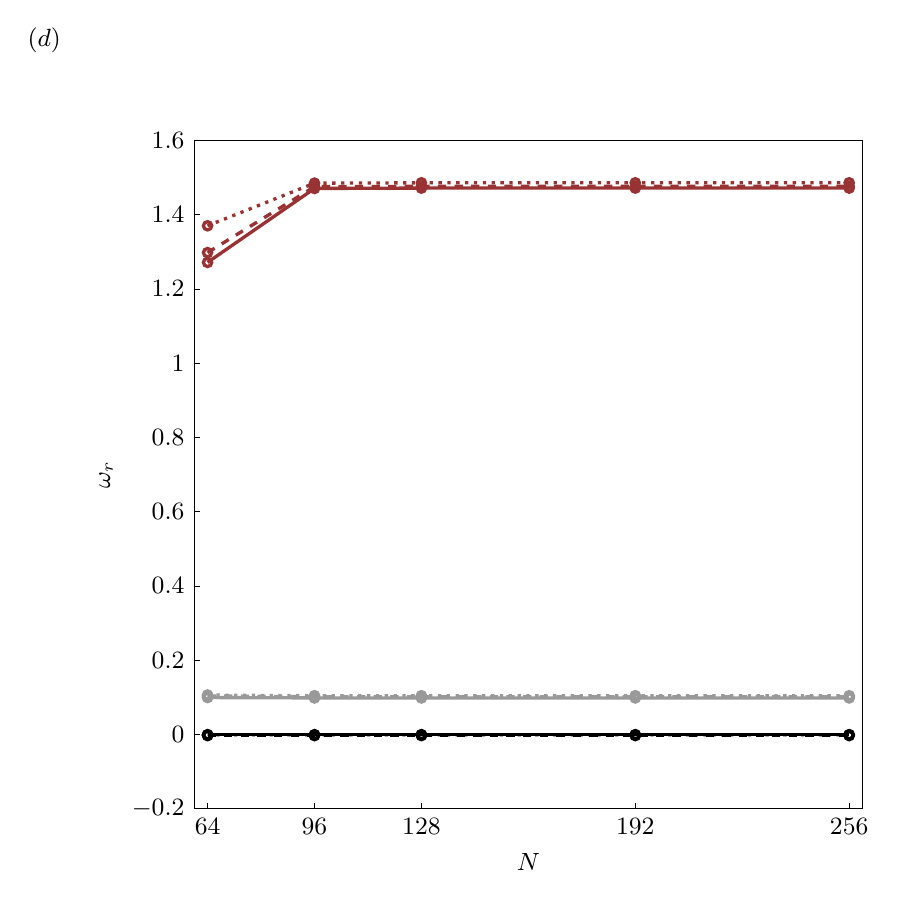
\begin{tikzpicture}

\begin{axis}[%
width=11.255in,
height=7.131in,
at={(1.888in,0.962in)},
scale only axis,
clip=true,
separate axis lines,
every outer x axis line/.append style={black},
every x tick label/.append style={font=\color{black}},
every x tick/.append style={black},
xmin=60,
xmax=260,
xtick={ 64,  96, 128, 192, 256},
xlabel={$N$},
every outer y axis line/.append style={black},
every y tick label/.append style={font=\color{black}},
every y tick/.append style={black},
ymin=-0.2,
ymax=1.6,
ylabel={$\omega_r$},
axis background/.style={fill=white},
clip=true,
clip mode=individual,
axis lines=box,
xtick pos=bottom,
ytick pos=left,
tick align=inside,
major tick length=2pt,
width=0.7\linewidth,
height=0.7\linewidth,
every axis/.append style={font=\fontsize{9}{9}\selectfont},xlabel style={font=\fontsize{9}{9}\selectfont},title style={font=\fontsize{9}{9}\selectfont},
legend style={font=\fontsize{8}{9}\selectfont,inner sep=1pt,row sep=1pt,column sep=2pt,nodes={scale=1.00},draw=none},legend image post style={xscale=0.35},
legend columns=1,
scaled x ticks=false,
tick label style={/pgf/number format/fixed,/pgf/number format/precision=2},
every x tick label/.append style={font=\fontsize{9}{9}\selectfont\color{black}},
every y tick label/.append style={font=\fontsize{9}{9}\selectfont\color{black}},
,,
colormap={sigmamap}{rgb(0.0000)=(0.0200,0.1880,0.3800); rgb(0.1000)=(0.0743,0.3456,0.5616); rgb(0.2000)=(0.1918,0.4980,0.7060); rgb(0.3000)=(0.3890,0.6708,0.8226); rgb(0.4000)=(0.7552,0.8682,0.9228); rgb(0.5000)=(0.9690,0.9689,0.9689); rgb(0.6000)=(0.9425,0.8044,0.7614); rgb(0.7000)=(0.8767,0.4910,0.4020); rgb(0.8000)=(0.7869,0.2866,0.2470); rgb(0.9000)=(0.6186,0.1239,0.1568); rgb(1.0000)=(0.4040,0.0000,0.1220)}
]
\addplot [color=black, line width=1.2pt, mark size=1.5pt, mark=o, mark options={solid, black}, forget plot]
  table[row sep=crcr]{%
64	-0.000993761100114939\\
96	-0.000993739398262548\\
128	-0.000993739950969389\\
192	-0.000993741127721846\\
256	-0.000993740340299722\\
};
\addplot [color=black, dashed, line width=1.2pt, mark size=1.5pt, mark=o, mark options={solid, black}, forget plot]
  table[row sep=crcr]{%
64	-0.00301354305557083\\
96	-0.00301358113240564\\
128	-0.00301358148008734\\
192	-0.00301359296872225\\
256	-0.00301358636765227\\
};
\addplot [color=black, dotted, line width=1.2pt, mark size=1.5pt, mark=o, mark options={solid, black}, forget plot]
  table[row sep=crcr]{%
64	-0.00107002281983706\\
96	-0.00106993448183487\\
128	-0.00106993482082553\\
192	-0.00106993676027198\\
256	-0.00106993805265659\\
};
\addplot [color=white!60!black, line width=1.2pt, mark size=1.5pt, mark=o, mark options={solid, white!60!black}, forget plot]
  table[row sep=crcr]{%
64	0.0993504663763069\\
96	0.0983478963248349\\
128	0.0983481750926426\\
192	0.0983481085839242\\
256	0.0983481682580654\\
};
\addplot [color=white!60!black, dashed, line width=1.2pt, mark size=1.5pt, mark=o, mark options={solid, white!60!black}, forget plot]
  table[row sep=crcr]{%
64	0.10379489905161\\
96	0.101561514617896\\
128	0.101561498537618\\
192	0.101561520528346\\
256	0.101561488021553\\
};
\addplot [color=white!60!black, dotted, line width=1.2pt, mark size=1.5pt, mark=o, mark options={solid, white!60!black}, forget plot]
  table[row sep=crcr]{%
64	0.106006960142888\\
96	0.104171461417367\\
128	0.104171464594514\\
192	0.104171514686636\\
256	0.104171468304152\\
};
\addplot [color=red!60!teal, line width=1.2pt, mark size=1.5pt, mark=o, mark options={solid, red!60!teal}, forget plot]
  table[row sep=crcr]{%
64	1.27134620738182\\
96	1.47047066019017\\
128	1.4714719844176\\
192	1.47146913484269\\
256	1.47146919294046\\
};
\addplot [color=red!60!teal, dashed, line width=1.2pt, mark size=1.5pt, mark=o, mark options={solid, red!60!teal}, forget plot]
  table[row sep=crcr]{%
64	1.29769172627066\\
96	1.47525986432074\\
128	1.47611362437013\\
192	1.47611533782889\\
256	1.47611531434549\\
};
\addplot [color=red!60!teal, dotted, line width=1.2pt, mark size=1.5pt, mark=o, mark options={solid, red!60!teal}, forget plot]
  table[row sep=crcr]{%
64	1.36990485224449\\
96	1.48475646855977\\
128	1.48563606891222\\
192	1.48563896383182\\
256	1.48563897911697\\
};
\node[right, align=left, inner sep=0]
at (rel axis cs:-0.25,1.15) {$(d)$};
\end{axis}
\end{tikzpicture}%